\chapter{\ac{IoT} Voting System Implementation} \label{chap:implementation}
\section{Hardware Setup}
The \ac{IoT} voting system comprises the following components:
\begin{itemize}
    \item \textbf{Tallier Node:} Sony Vaio E Series laptop (Intel Core i5-2450M, 8 GB DDR3 RAM) running Antix Linux 23.1, serving three critical roles:
    \begin{itemize}
        \item Wi-Fi \ac{AP} (using hostapd v2.9)
        \item MQTT Broker (using Eclipse Mosquitto v2.0.20)
        \item Election Tallier
    \end{itemize}
    \item \textbf{Guardian Nodes:} 2× NodeMCU ESP32 boards (ESP32-WROOM-32 modules) with:
    \begin{itemize}
        \item 240 MHz dual-core Xtensa LX6 CPU
        \item 520 KB SRAM, 4 MB flash
        \item Integrated 802.11 b/g/n Wi-Fi
    \end{itemize}
\end{itemize}
The Guardian nodes are responsible for distributing trust in the encryption and decryption processes managed by the Tallier. 

\section{Election Setup} \label{sec:constants}
The Guardian nodes responsibilities are divided into two main phases: the key-generation ceremony, and the decryption process.

Before implementing the ElectionGuard specification, it is essential to establish the mathematical constants for the cryptographic operations. ElectionGuard specifies standard values for the primes (p) and (q) and a generator (g) \cite[21]{eg-spec}. The standard baseline parameters include:
\begin{itemize}
    \item A 4096-bit prime (p) \cite[22]{eg-spec}
    \item A 4096-bit generator (g) \cite[23]{eg-spec}
    \item A 256-bit prime (q) \cite[21]{eg-spec}
\end{itemize}

For this experiment, we will use reduced parameters that offer better performance at a lower security level \cite[23]{eg-spec}. The reduced parameters are defined as  
\begin{itemize}
    \item A 3072-bit prime (p) \cite[36]{eg-spec}
    \item A 3072-bit generator (g) \cite[36-37]{eg-spec}
    \item A 256-bit prime (q) \cite[36]{eg-spec}
\end{itemize}

\subsection{Pre-Election Key-generation}
The pre-election phase involves administrative tasks necessary to configure the election, including the key-generation ceremony.

\begin{figure}
    \centering
    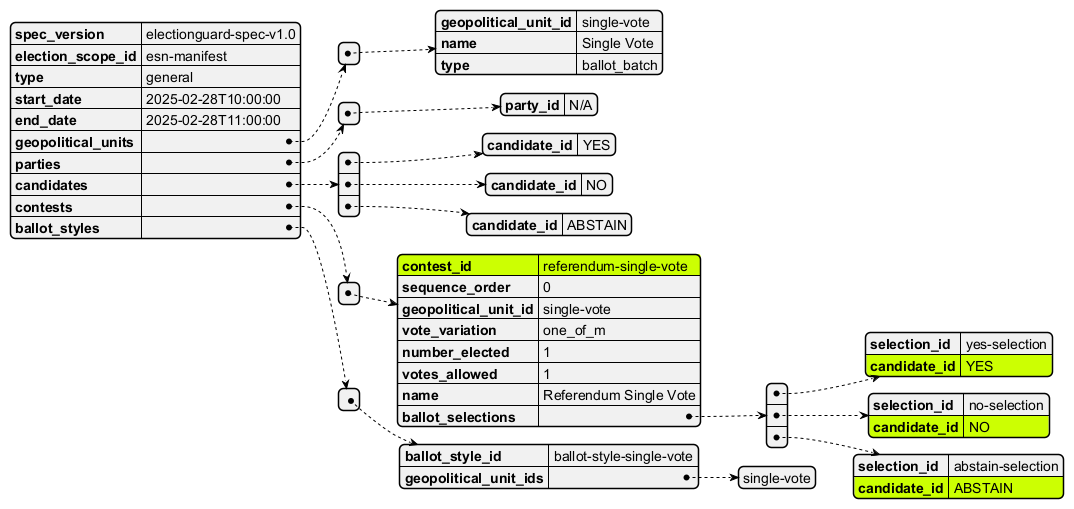
\includegraphics[width=\textwidth]{abbildungen/Diagramme/manifest.png}
    \caption{Visualisation of the JSON Election Manifest}
    \label{Fig:manifest}
\end{figure}

The tallier node defines the election manifest, sets the cryptographic constants according to the reduced baseline parameters (as discussed in \ref{sec:constants}), and sets the quorum size. Given that only two Guardian nodes are available for this experiment the quorum size is set to two. Figure \ref{Fig:manifest} shows a visualisation of the election manifest used in this election. The election is limited to a simple YES/NO/ABSTAIN referendum. The Tallier collaborates with the Guardians to generate a joint key used to encrypt the ballots in the next election phase.

\begin{figure}
    \centering
    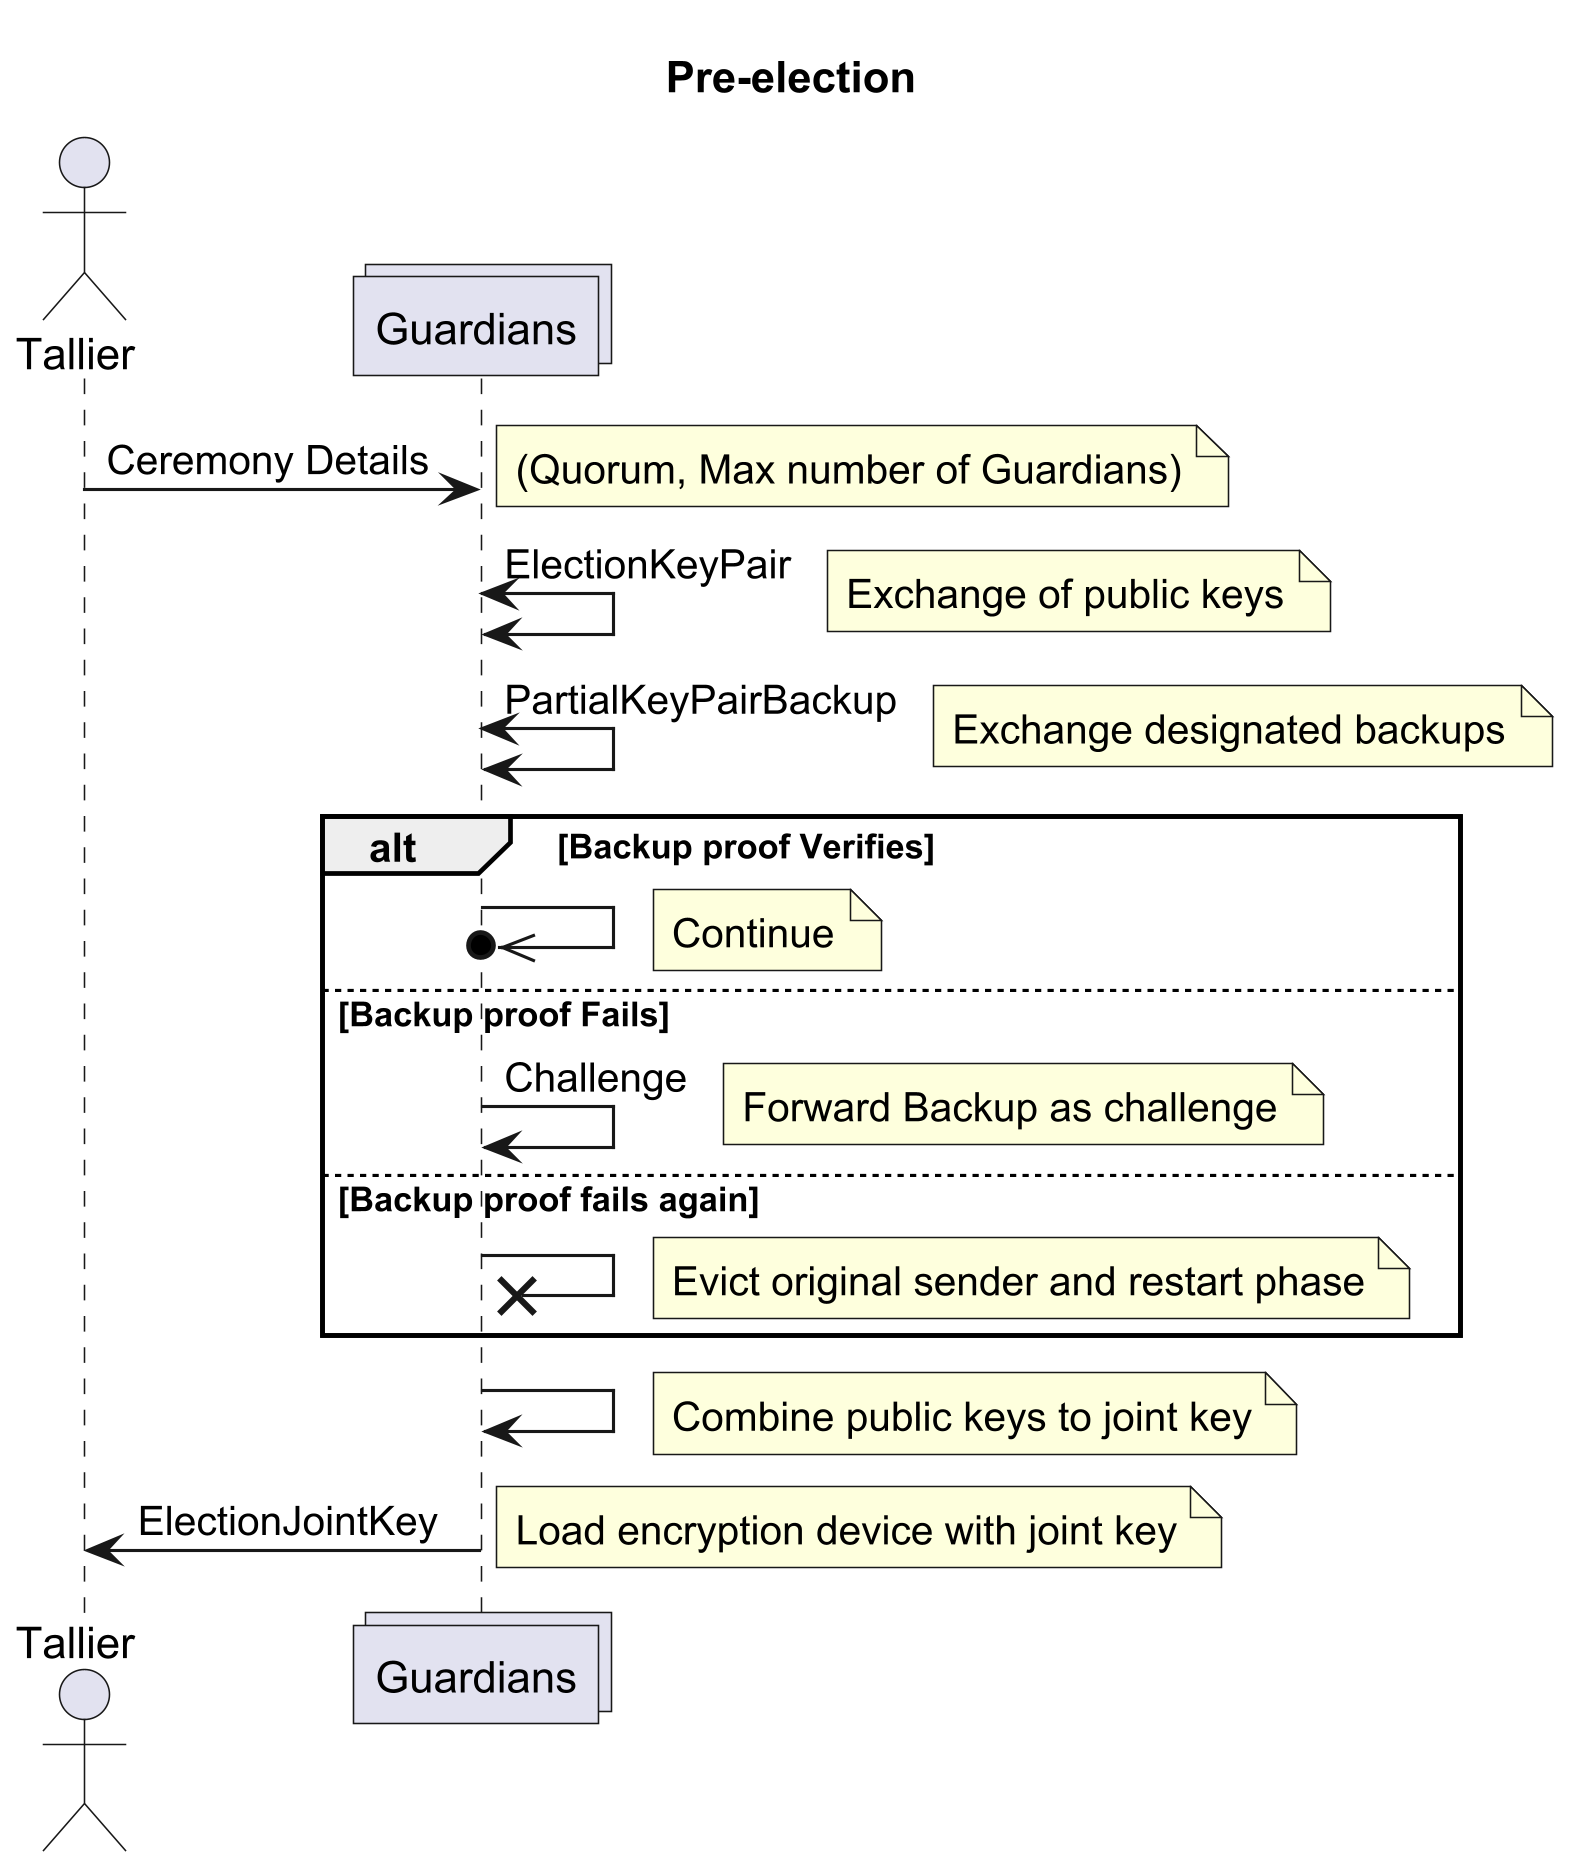
\includegraphics[width=0.7\textwidth]{abbildungen/Diagramme/communication-seq0.png}
    \caption{Communication Sequence in the Pre-election phase}
    \label{Fig:comm-pre}
\end{figure}

Figure \ref{Fig:comm-pre} illustrates the communication sequence involved in this phase. The Tallier sends the ceremony details required for the key-generation ceremony to the Guardians. The quorum size influences how each Guardian generates their ElectionKeyPair. After generating their ElectionKeyPair and stripping the secret key for transmission, the Guardians exchange their ElectionKeyPairs. Each Guardian generates a designated backup for each ElectionKeyPair received, which is then sent back to the sending Guardian. Each backup contains a proof that must be verified by the receiver. Once all backups successfully verify, the ElectionKeyPairs are combined into a joint key. The challenge mechanism and eviction mechanism for failed verifications are not implemented in this experiment. ElectionGuard assumes the key-generation runs between publicly identified parties, and there is little benefit for a malicious participant in introducing errors. Therefore, it is assumed that Guardians abort the key-generation as soon as one of them detects an error, restarting the protocol from scratch, possibly replacing Guardians that are identified as acting maliciously \cite[9]{eg-paper}. 

\subsection{Intra-Election Ballot Encryption}
During this election, the Tallier simulates the voting process by generating random ballots and encrypting them using the joint key established in the previous phase. In the example in the Appendix \ref{lst:ballotgen} the Tallier generates 10 ballots and encrypts them. We test the configuration with 10, 100 and 1000 ballots.

\subsection{Post-Election Decryption of Tallies}
In the post-election phase, all encrypted ballots from the previous phase are homomorphically aggregated to produce an encrypted tally. This encrypted tally is sent to the Guardians for decryption. Each guardian uses their private key to generate a decryption share, which is essentialy a partial decryption. The Tallier then combines all decryption shares into a decrypted tally. Figure \ref{Fig:comm-post} illustrates the communication involved in this phase. The decryption of spoiled ballots is optional and not implemented in this experiment. The decryption process of the spoiled ballots mirrors that of the encrypted tally. The case of missing Guardians is also not addressed in this experiment. Compensating for missing decryptions functions similarly to the generation of the decryption share. The publication of the election artifacts is also not implemented, the interaction between the Guardian and the Tallier requires inherent verification due to the proofs involved as seen in Appendix \ref{lst:proof}.

\begin{figure}
    \centering
    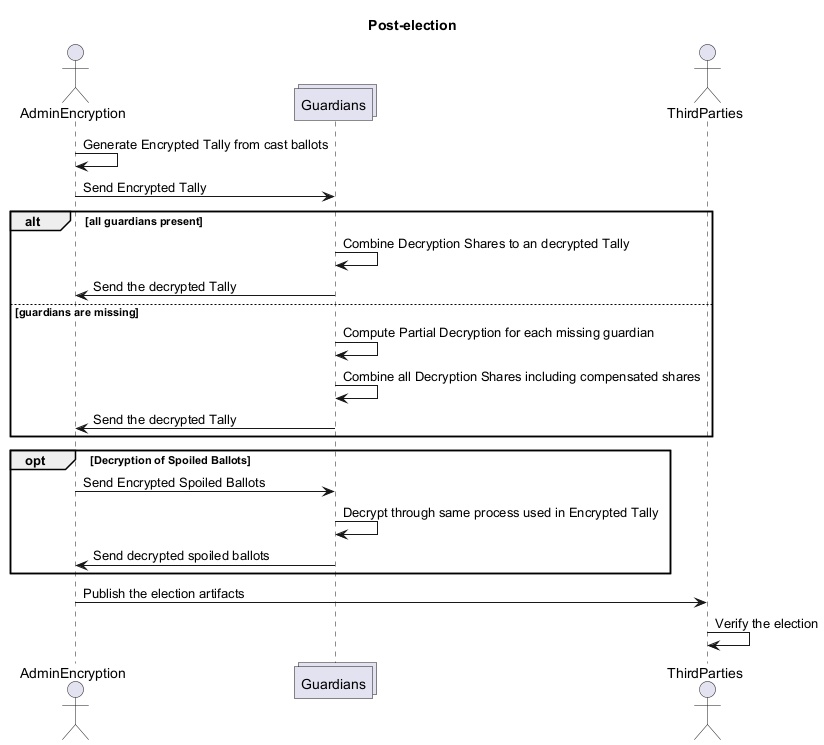
\includegraphics[width=0.7\textwidth]{abbildungen/Diagramme/communication-seq2.png}
    \caption{Communication Sequence during the Pre-Election Key-Generation Ceremony}
    \label{Fig:comm-post}
\end{figure}

\section{Comparison of ElectionGuard Implementations}
Due to the open-source nature of ElectionGuard, various community ports exist, such as a Java port \cite{eg-docs}. However, this discussion focuses solely on the official ports from Microsoft. There are 2 ElectionGuard libraries implementing the ElectionGuard 1.0 specification: a Python reference implementation and a C++ reference implementation. The Python implementation encompasses the entire suite of functionality and processes necessary to implement \ac{E2E} verifiable election as part of a voting system \cite{python-reference}. It is designed to be universal and portable, albeit less performant \cite{eg-docs}. In contrast, the C++ reference implementation focuses solely on the encryption components and is optimised for execution on low-powered devices \cite{cpp-reference}. 

\subsection{Python Reference}
Running the Python reference implementation on the ESP32 may be feasible through \textbf{MicroPython}, an implementation of Python 3.x targeted for microcontrollers and embedded systems. MicroPython adapts standard Python library functionalities to accommodate the limitations inherent of microcontrollers, such as restricted memory and processing speed \cite{micropython} \cite[234]{micropython-performance}. There are drawbacks to this approach, as essential modules, functions, and classes may be absent in MicroPython \cite{micropython}. Additionally, applications developed in MicroPython are prone to memory fragmentation and may experience issues with objects expending in size. \cite[234]{micropython-performance}. A comparative study of software-based \ac{SHA}-256 computation for the ESP32 revealed that the performance of MicroPython was inferior to that of a C implementation \cite[237]{micropython-performance}. For instance, the C implementation outperformed the MicroPython implementation by 45\% \cite[237]{micropython-performance}.

The Electionguard Python reference is not designed to be performant, and compatibility issues may arise when using MicroPython, along with potential memory fragmentation problems. Due to these limitations, the Python reference implementation may not be the most suitable choice for the ESP32. However, it remains a valuable resource for understanding the ElectionGuard specification and can serve as a reference for developing a possible port. Our Tallier node, which has more computational resource compared to our Guardians, will run the Python reference implementation as a Python package for convenience.

\subsection{C++ Reference}
The ElectionGuard C++ reference implements focuses solely on the encryption library, omitting abstractions such as Guardians. This implementation is designed for execution on low-powered devices with Intel Atom-level processor performance in mind \cite{cpp-reference} \cite{eg-docs}. Porting the C++ library to an ESP32 should be feasible, as ESP-IDF supports C++ application development. Certain C++ features, such as exception handling, must be enabled in the project configuration beforehand. The ESP32 also supports C++ threads, which are implemented as wrappers around C pthreads, which in turn wrap around FreeRTOS tasks \cite{esp-prog}. 

Compared to the Python implementation, the C++ implementation incorporates optimisations to accelerate computations of certain modular exponentiations \cite{cpp-reference}. These optimisations come at a memory cost. The optimisation for modular exponentiation uses pre-computed tables to speed up calculations for certain exponentiations \cite{cpp-reference}. A modular exponentiation computes \(X^Y \bmod P\). This optimisation is possible because many of the exponentiations in ElectionGuard are performed with a fixed base, such as the generator (g). The pre-computed table contains certain powers of these bases, allowing the computation \(G^Y\) to be turned into a series of table lookups \cite[22-23]{eg-paper}.

To store the table, we must consider the capabilities of the ESP32. The ESP32 has 520 KB of volatile memory (SRAM) and 4 MB of non-volatile memory (in-package flash). The SRAM is divided into 320 KB of DRAM and 200 KB of IRAM. IRAM is used for instruction memory, while DRAM is used for data memory. The maximum statically allocated DRAM usage is 160 KB, the remaining 160 KB can only be allocated as heap memory \cite{esp32-ref}. 

\begin{lstlisting}[language=C++, caption={FixedBaseTable Definition from \cite{cpp-reference}}]
    typedef std::array<std::array<uint64_t[MAX_P_LEN], OrderBits>, TableLength> FixedBaseTable;
\end{lstlisting}

The lookup table (FixedBaseTable) is implemented and tuned to the following values. Any modifications to these parameters could affect the function's internal operations \cite{cpp-reference}.
\begin{itemize}
    \item b= 256 (OrderBits) \cite{cpp-reference}.
    \item k = 8 (WindowSize) \cite{cpp-reference}.
    \item m = 32 (TableLength) \cite{cpp-reference}.
\end{itemize}

To estimate the memory requirements of the \textbf{FixedBaseTable}, we can calculate the total size in bytes as follows:
\begin{equation}
    \mathrm{FixedBaseTable Size} = \mathrm{sizeof(uint64\_t)} \times \mathrm{MAX\_P\_LEN} \times \mathrm{OrderBits} \times \mathrm{TableLength}
\end{equation}
Given that MAX\_P\_LEN is defined as 64 (4096-bit), we will calculate with 48 (3072-bit) since we are using the reduced baseline parameters. Substituting the values into the equation gives:
\begin{equation}
    \mathrm{FixedBaseTable Size} = 8 \times 48 \times 256 \times 32 =  3145728  \mathrm{ bytes} = 3 \mathrm{ MB}
\end{equation}

Consequently, the \textbf{FixedBaseTable} exceeds the volatile memory capacity of the ESP32. Although storing the table in the non-volatile memory might be feasible, it may require further optimisations because it must accommodate the bootloader and the application binary. Reducing the \textbf{WindowSize} would result in smaller tables and reduced memory usage, but it simultaneously increases the number of multiplications \cite[22]{eg-spec}. Given these memory requirements, it is evident that the C++ implementation would require further optimisations to be feasible on the ESP32. Therefore, we opt to implement a native C implementation based on the Python reference implementation.

\subsection{Implementation Strategy for ESP32}
ElectionGuard uses integer ElGamal cryptography within its specific cryptographic operations. The system performs four key operations on very large integer values: \textbf{modular exponentiation}, \textbf{modular multiplication}, \textbf{modular addition}, and \textbf{SHA-256} hash computation \cite[25]{eg-spec}. 

To handle the large integer values involved in these operations, specialised libraries for large integers may be employed, or the operations can be developed from scratch \cite[21, 25-26]{eg-spec}. When developing these modular operations from the ground up, it is common for intermediate values to become excessively large. Techniques such as modular reduction are often necessary to ensure that values remain manageable \cite[21, 25-26]{eg-spec}. Consequently, employing fast libraries for modular arithmetic becomes crucial for achieving good performance \cite[22]{eg-paper}. The Python implementation uses the C-coded GnuMP library \cite{python-reference} for large integer arithmetic, the C++ implementation uses HACL* a performant C implementation of a wide variety of cryptographic primitives \cite[22]{eg-paper} \cite{cpp-reference}. In ESP32 cryptographic primitives are implemented through a fork of the mbedTLS library. Optionally, a port of the WolfSSL library is also available \cite{esp32-ref}. The benefit of these two libraries over the other mentioned libraries is that these libraries include patches related to hardware routines for on-board cryptographic hardware acceleration \cite{esp32-ref} \cite[114]{wolfSSL-manual}. The ESP32 supports supports several cryptographic hardware acceleration capabilities including \ac{AES}, \ac{SHA}, \ac{RSA}, and \ac{RNG} as illustrated in the functional block diagram \ref{Fig:esp32-crypto}. These hardware accelerators significantly enhance operational speed and reduce software complexity for the aforementioned cryptographic primitives \cite[32]{esp32-series}. More details on the hardware acceleration capabilities of the ESP32 are provided in section \ref{sec:hardware-acceleration}.

\begin{figure}
	\centering
	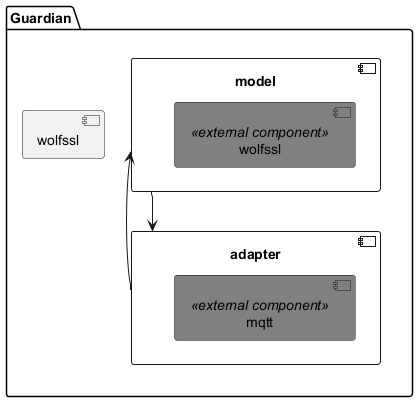
\includegraphics[scale=.5]{abbildungen/Diagramme/components.png}
	\caption{Software components for the Guardian Prototype}\label{Fig:software-components} 
\end{figure}

Figure \ref{Fig:software-components} depicts the software components used in the Guardian ESP32 port. The model component includes the business logic for the Guardians operations. The adapter component implements the communication aspects. The adapter component calls the model component to perform guardian specific operations. The model component uses the wolfSSL library for cryptographic primitives. The wolfSSL component is overwritten using C pre-processor macros to reduce the binary size by removing unused features. Furthermore, the library is configured to run on the memory-restricted ESP32 by configuring the library to use less memory, albeit at a performance cost \cite[56-58]{doxygen}. The adapter component implements a \ac{MQTT} client. It is used in order to communicate with the Tallier and other Guardians through an intermediary the \ac{MQTT} broker. The adapter component implements an event handler which response to events such as establishing a connection to the \ac{MQTT} broker or receiving a message via the \ac{MQTT} broker. Further information on the implementation of the adapter component and the communication can be found in section \ref{sec:communication}. 

\section{Hardware Acceleration} \label{sec:hardware-acceleration}
ElectionGuard encryption is fundamentally a CPU-bound operation \cite[24]{eg-paper}. The ESP32 microcontroller features hardware acceleration for several cryptographic primitives, including \ac{AES}, \ac{SHA}, \ac{RSA}, and \ac{RNG} \cite{esp32-ref}. These hardware accelerators significantly enhance the performance of cryptographic operations compared to software implementations \cite[32]{esp32-series}. By offloading cryptographic operations from the CPU, these accelerators reduce computational load and improve overall system performance \cite[32]{esp32-series}. They are particularly beneficial for computationally intensive operations, such as modular exponentiation and modular multiplication, which are central to the ElectionGuard encryption process \cite[24]{eg-paper}. The following sections explore how each hardware accelerator can be utilised in the ElectionGuard implementation.

\subsection{\ac{RNG}}
In ElectionGuard, generating random values is crucial for various operations, including the key-generation and nonce usage in various proofs \cite[9, 13]{eg-spec}. The ESP32 features a \ac{TRNG} that produce 32-bit random numbers that are suitable for cryptographic purposes. Unlike \ac{DRBG}, which rely on algorithms to produce random numbers, the ESP32's \ac{TRNG} generates randomness from physical processes, such as thermal noise and asynchronous clock mismatches. This ensures a high level of unpredictability essential for cryptographic operations \cite[604]{esp32-ref}. To effectively utilise the \ac{TRNG}, a source of thermal noise must be enabled; otherwise, the \ac{TRNG} will return pseudo-random numbers \cite[609]{esp32-ref}. The high-speed \ac{ADC} is automatically enabled when the Wi-Fi or Bluetooth module is active. When sourcing noise from the high-speed \ac{ADC}, it is advisable to read the \textbf{RNG\_DATA\_REG} register at a maximum rate of 5 MHz \cite[609]{esp32-ref}. Extreme conditions can lower the resulting entropy. To mitigate this, enabling the \textbf{SAR\_ADC} as a secondary noise source is recommended. The \textbf{RNG\_DATA\_REG} register should then be read at a maximum rate of 500 kHz to obtain the maximum entropy \cite[609]{esp32-ref}.

In the ESP32 Guardian implementation, the \textbf{rand\_q} function generates a random number below the constant 256-bit constant (q). A 256-bit buffer is filled with randomness from the \ac{TRNG} using the ESP32 system API. To ensure the generated 256-bit number does not exceed (q) a modulo operation is performed with the value of (q). The 32-bit \textbf{RNG\_DATA\_REG} is read eight times to fill the 256-bit buffer. The system API function will delay if the reading frequency exceeds the maximum reading rate. This delay is necessary to ensure that sufficient external entropy has been introduced into the hardware \ac{TRNG} state \cite{esp32-ref}. Alternatively, using a strong software \ac{DRBG} can be initialised with the \ac{TRNG} values as a seed \cite{esp32-ref} \cite[588]{wolfSSL-manual}. In this implementation the the risks of delays are neglibile since the reading frequency is low.

\subsection{\ac{SHA} Accelerator}
In ElectionGuard, hashes are computed using the \ac{SHA}-256 hash function \cite[26]{eg-spec}. The implementation requires caution because all inputs, whether textual or numeric, are represented as utf-8 encoded strings \cite[26]{eg-spec}. In our case, this is less efficient than hashing the raw bytes of the large integer values due to the conversion overhead to convert the large integer values to utf-8 encoded strings before hashing. This is necessary to get hash value consistent with the Python implementation. The \ac{SHA}-256 hash function is frequently applied in various cryptographic operations within ElectionGuard. For example, non-vote data such as a Guardians backup share don't need to be homomorphically encrypted. Instead, they are encrypted using hashed ElGamal encryption \cite[7]{eg-spec}. The function hashed ElGamal encryption uses a \ac{KDF} based on \ac{HMAC} that is instantiated with SHA-256 (HMAC-SHA-256) \cite[7]{eg-spec}. 

The \ac{SHA} Accelerator significantly enhances the performance of \ac{SHA} operations compared to purely software implementations \cite[589]{esp32-ref}. This accelerator support the \ac{SHA}-256 algorithm used in the ElectionGuard specification. It processes one 512-bit message block at a time. Therefore, software must manage the division of longer messages, along with any required padding \cite[2]{esp32-series}. In multi-core environments, libraries like mbedTLS and WolfSSL implement fallback mechanisms to software when concurrent hashing operations are initiated. As a result, computations revert to software calculations when the hardware accelerator is busy \cite{mbedTLS-fork} \cite{wolfSSL-port}. Benchmarks utilising mbedTLS at processor speeds of 240 MHz reveal that hardware acceleration achieves performance nearly three times faster than the software counterpart \cite[41-42]{eval-crypto}. Thus, the \ac{SHA} Accelerator is an effective solution for speeding up \ac{SHA}-256 hashing operations on the ESP32.


\subsection{\ac{RSA} Accelerator}
ElectionGuard's decision to use integer ElGamal instead of elliptic-curve ElGamal was driven by its conceptual simplicity and lower implementation barrier \cite[7]{eg-paper}. While \ac{ECC} techniques offer computational advantages, such as reduced computing requirements and smaller key sizes for the same security level \cite[1, 6]{ecc-eval}, the integer ElGamal approach aligns well with the ESP32 hardware. This is because the \ac{RSA} algorithm, like integer ElGamal, relies on large integer arithmetic. Specifically, the ESP32 chip supports independent arithmetic operations, including large-number multiplication, large-number modular multiplication, and large-number modular exponentiation \cite[32]{esp32-series} \cite[603]{esp32-ref}. Consequently, the RSA Accelerator can accelerate two key ElectionGuard operations: modular multiplication and the computationally intensive modular exponentiation. The RSA Accelerator supports operand lenghts of up to 4096 bits \cite[603]{esp32-ref}, which is sufficient for the reduced and standard baseline parameters used in ElectionGuard. A modular exponentation computes \( Z = X^Y \bmod M \), while modular multiplication computes \( Z = X \times Y \bmod M \). Both operations are based on Montgomery multiplication. In addition to the input arguments \( X \), \( Y \), and \( M \), two additional arguments are required: the Montgomery Inverse \( \overline{r} \) and the inverse of M \( M' \). These additional arguments are precomputed by software \cite[598-599]{esp32-ref}. 

Benchmarks comparing the modular exponentation using the mbedTLS library reveal that hardware acceleration is more than 12.84 times faster than software implementations \cite[51]{eval-crypto}. However, for small operands the hardware acceleration was 1.44 times slower than the software implementation. This is likely due to the initialisation overhead of the hardware accelerator outweighing the benefits for smaller values \cite[51]{eval-crypto}. Initialisation with small values occurs during the polynomial calculation used in the key-generation. The number of polynomials (starting from 0 and incrementing) is used as the exponent in the operation. Therfore, this penalty could effect us. However, the wolfSSL library used in the ESP32 implementation fallbacks to the software implementation for small operands. Sadly, the mbedTLS has one benefit over the wolfSSL library in that it allows caching of the \( \overline{r} \) and \( M' \) values, which can significantly speed up operations \cite[51]{eval-crypto}. Due to the fact that all M values are either (q) or (p) and thus constant throughout the computations, caching the \( M' \) is likely to be beneficial due to the avoiding of recalculating the inverse of M each time. The \( \overline{r} \) can also be cached. \( \overline{r} \) is calculated as \( R^2 \bmod M \) where R is calculate as \(2^{n \cdot 32 \cdot 2}\). (n) is the number of 32-bit words in M.

In summary, the \ac{RSA} Accelerator effectively accelerates modular exponentiation and modular multiplication in the ElectionGuard implementation. The mbedTLS library might be a better choice due to the caching of the \( \overline{r} \) and \( M' \) values. But a fallback mechanism for small operands is necessary to avoid inefficiencies when using the \ac{RSA} Accelerator with small values. 

\subsection{Performance Analysis}
ElectionGuard perform essentialy four key operations on very large integer values: \textbf{modular exponentiation}, \textbf{modular multiplication}, \textbf{modular addition}, and \textbf{SHA-256} hash computation \cite[25]{eg-spec}. Using the previously discussed hardware accelerators, the performance of the ElectionGuard operations can be significantly improved. The \ac{RSA} Accelerator can accelerate the computationally intensive modular exponentiation and modular multiplication operations. The \ac{SHA} Accelerator can speed up the \ac{SHA}-256 hash computation. The modular addition cannot be accelerated using dedicated hardware and must rely on a software implementation. The \ac{TRNG} is only used as a entropy source for generating random numbers and does not accelerate any cryptographic operations.

\begin{table}[h!]
    \centering
    \begin{tabular}{|c|c|c|c|}
        \hline
        \textbf{Quorum} & \textbf{Type} & \textbf{Average Time (s)} & \textbf{Standard Deviation (ms)} \\
        \hline
        Quorum 2 & HW & 1.02 & 0.24 \\
        & SW & 4.41 & 13.24 \\
        \hline
        Quorum 3 & HW & 1.53 & 0.23 \\
        & SW & 6.62 & 15.87 \\
        \hline
        Quorum 4 & HW & 2.03 & 0.24 \\
        & SW & 8.81 & 15.68 \\
        \hline
        Quorum 5 & HW & 2.54 & 0.26 \\
        & SW & 11.02 & 19.15 \\
        \hline
        Quorum 6 & HW & 3.05 & 0.31 \\
        & SW & 13.22 & 22.04 \\
        \hline
    \end{tabular}
    \caption{Comparison accelerated (HW) and non accelerated (SW) key-generation with different Quorums, 30 measurements}
    \label{tab:perfromance-quorum}
\end{table}

\begin{table}[h!]
    \centering
    \begin{tabular}{|c|c|c|c|c|}
        \hline
        \textbf{Function} & \textbf{Type} & \textbf{Average Time (s)} & \textbf{Standard Deviation (ms)} \\
        \hline
        Backup & HW & 0.53 & 0.15 \\
        & SW & 2.21 & 8.52 \\
        \hline
        Verification & HW & 1.06 & 0.1 \\
        & SW & 2.58 & 0.04 \\
        \hline
        Decryption & HW & 2.29 & 1.61 \\
        & SW & 9.95 & 19.4 \\
        \hline
    \end{tabular}
    \caption{Comparison of operations with (HW) and without (SW) hardware acceleration, 30 measurements}
    \label{tab:perfromance}
\end{table}

Test software was written to measure the performance of the the pre-election key-generation ceremony operations and the post-election decryption operations. The key-generation ceremony operations tests the key-generation with different quorums, the backup generation, and the verification of the backups. The post-election decryption operations tests the decryption of the encrypted tally. The decryption is performed with 1 contest and 3 selections (e.g., YES/NO/ABSTAIN). The test measures only the time taken to complete the operation and does not include any prior parameter initialisation. The test performs each operation 30 times to obtain an average time. The standard deviation was also calculated to measure the dispersion of the measurements relative to the mean. High standard deviation values indicate a more variable performance. Each operation was performed after a cold boot of the ESP32 to ensure that the results were not influenced by any prior operations. The software was compiled with the -O2 GCC optimisation flags to optimise compilation for speed. For the software-only runs the hardware acceleration was disabled by setting specific wolfSSL C-preprocessor macros. Table \ref{tab:perfromance-quorum} compares the performance of accelerated key-generation (HW) and non-accelerated key-generation (SW) across different quorums. Table \ref{tab:perfromance} summarises the performance of hardware-accelerated operations (HW) versus without (SW) across three tasks: decryption, verification, and backup. 

The results of \ref{tab:perfromance-quorum} indicate that the accelerated operations (HW) are more then four times faster than purely software operations (SW) across all quorum sizes (e.g., 1.02s vs. 4.41s for Quorum 2). HW shows remarkably low standard deviations (0.23-0.31ms)  compared to SW (13.24-22.04ms). This indicates that accelerated operations have a more stable, consistent performance. Large quorums provide better security but at the cost of increased computational time. The average time for the accelerated oporation increase by ~0.5s per additional quorum member (1.02s → 3.05s from Q2→Q6). The SW implementation shows a similar trend, but with a steeper increase by ~2.2s per additional member (4.41s → 13.22s from Q2→Q6). This suggest O(n) complexity for both implementations. Table \ref{tab:perfromance} indicates that the accelerated backup operation (0.53s vs. 2.21s) and the accelerated decryption operation  (2.29s vs. 9.95s) is more than four times faster. The accelerated verification operation is more than twice as fast as the SW implementation. Accelerated operations show again a more stable performance with lower standard deviations compared to non-accelerated operations. The speedup of the verification is likely less pronounced due to the initial computation steps using small values and thus executing with the software implementation. These results underscore the efficacy of hardware accelerators in optimising both the speed and reliability of cryptographic workflows.  


\section{Communication}\label{sec:communication}
The laptop is configured as an \ac{AP}, enabling its wireless interface to create a local Wi-Fi network. This communication range is limited by the Wi-Fi signal strength of the laptop's \ac{AP}. However, the entire system portable as long as the laptop and the connected \ac{IoT} devices are powered. Our \ac{IoT} devices-The NodeMCU ESP32 development boards-are connected to the \ac{AP}. \ac{IoT} systems rely primarily on using messaging protocols for exchanging \ac{IoT} data and there exists several protocols or frameworks that support distinct types of messaging patterns . Given that \ac{IoT} devices typically have limited computational resources and processing power, choosing a lightweight, reliable, scalable, interoperable, extensible and secure messaging protocol becomes a very
challenging task. \cite[1]{protocols}.

\subsection{Data Link Layer Protocols}
When selecting an appropriate messaging protocol for \ac{IoT} devices, it is essential to consider the hardware characteristics of these devices and the types of data link layer protocols they support. The data link layer is responsible for facilitating data transfers between network entities \cite[1-3]{protocols}. For instance, the ESP32 microcontroller supports both Wi-Fi and Bluetooth data link layer protocols \cite{esp-prog}. The Bluetooth system on the ESP32 can be further divided into Classic Bluetooth and \ac{BLE} \cite{esp-prog} \cite{esp-faq}. Both Wi-Fi and Bluetooth can operate simultaneously, but this requires time-sharing control \cite[77]{esp-faq}. There are additional networking protocols built on top of Wi-Fi and \ac{BLE}. Both Wi-Fi and \ac{BLE} support mesh networking, which facilitates many-to-many device communication and is optimised for creating large-scale device networks. The Wi-Fi stack also supports the proprietary ESP-NOW protocol, which allows direct device-to-device communication with ESP32 devices without requiring an \ac{AP} connection \cite{esp-prog}.

The throughput of \ac{IoT} devices can vary significantly based on the bandwidth they support. Since there is no universal radio technology for \ac{IoT} devices, the physical data rates they can achieve depend heavily on their size and hardware components \cite[1-2]{protocols}. Additionaly, throughout can be influenced by various factors, including environmental interference, connection intervals, and the size of the \ac{MTU} \cite{esp-faq}. The maximum \ac{BLE} throughput achievable on the ESP32 is about 90 KB/s, for Classic Bluetooth is about 200 KB/s, and for Wi-Fi it is about 20 MBit/s TCP and 30 MBits/ UDP \cite[38, 58,71]{esp-faq} \cite[2666]{esp-prog}. Understanding protocols at the data link layer is not sufficient for build \ac{IoT} applications. It is essential to also consider the protocols that exist at the application level, which complement those at the data link layer. While all messaging protocols facilitate data communication between entities via a transmission medium, their characteristics vary. Understanding how these protocols operate and addressing potential challenges is essential for identifying a suitable protocol. A well-suited messaging protocol can help reduce network traffic and latency, thereby enhancing the reliability of an \ac{IoT} application \cite[2,15]{protocols}. 

Within the ESP32 microcontroller, several application layer protocols address a wide range of application requirements. Modbus, for example, is a protocol primarily used in industrial \ac{IoT} environments \cite[3]{protocols} \cite{esp-prog}. ESP also supports the HyperText Transfer Protocol (HTTP) and the \ac{MQTT} protocol \cite{esp-prog}. 

\begin{comment}
    Distance. Limited by access point
    Wi-Fi (802.11n) generally has a higher transmission range of up to approximately 1 km compared to \ac{BLE}, which has a range of up to approximately 100 m \cite[3]{protocols}. 

    To facilitate Device-to-Device communication the laptop is configured as an MQTT broker using Eclipse Mosquitto version 2.0.20. It is important to note that this setup is not purely Device-to-Device communication, as it relies on the MQTT broker as an intermediary. Chapter \ref{sec:communication} describes the communication aspects in more detail.

    However, it is important to note that \ac{NAN} Datapath security is not supported, meaning that data packets cannot be encrypted, making it less suitable for transmitting sensitive information \cite[2694]{esp-prog}.
\end{comment}

\section{Communication Factors}
In the following sections we will look into communication factors that influence the choice of messaging protocol for the proposed voting system.

\subsection{Payload Size}
One important aspect that narrow down the choice of messaging protocols is the maximum payload size. For each payload we send in order to demonstrate that the payload was computed correctly we add a \ac{ZK} proof that allows the receiving party to verify the correctness of the payload without revealing any additional information (e.g., secret key) \cite[13]{stuve-study}. Proofs consist of commitments, challenge and response values. Challenge and response values take up 32 bytes in size each \cite[23]{eg-paper}.

At the post-election decryption phase Guardians send the decryption share to the Tallier. The decryption share is accompanied by Chaum-Pedersen proofs for each selection in a contest. In our experiment we have one contest with 3 selections YES/NO/ABSTAIN. Thus, the decrpytion share contains 3 Chaum-Pedersen proofs. The commitment of the Chaum-Pedersen proof is 1024 bytes (standard parameters) or 768 bytes (reduced parameters) in size. The minimum size of the Chaum-Pedersen proof is thus 1088 bytes (standard parameters) or 832 bytes (reduced parameters) in size. A contest with 3 selection would thus require 3264 bytes (standard parameters) or 2496 bytes (reduced parameters) in size.

During the pre-election key-generation the Guardians share private key shares among each other. This allows a quorum of Guardians to decrypt the election results without needing to reconstruct the private keys of missing Guardians. These shares are accompanied by Schnorr proofs too ensure the receiving Guardians can confirm the shares they receive are meaningful \cite[9]{eg-spec}. The quorum size of this experiment is 2 Guardians, thus each Guardian would need to generate 2 Schnorr proofs, one for each Guardian. The commitment of a SchnorrProof is 512 bytes (standard parameters) or 384 bytes (reduced parameters) in size. A Schnorr proof is thus 576 bytes (standard parameters) or 448 bytes (reduced parameters) in size. The total size of a Guardians Schnorr proofs for a Quorum of 2 Guardians is 1152 bytes (standard parameters) or 896 bytes (reduced parameters). 

Maximum packet size at the application layer:
\begin{itemize}
    \item \ac{BLE} Mesh Network: 384 bytes \cite[35]{esp-faq}
    \item Wi-Fi Mesh Network: 1456 bytes \cite[54]{esp-faq}
    \item ESP-NOW: 250 bytes \cite[47]{esp-faq}
    \item \ac{MQTT}: 265 MB \cite[16]{protocols}
    \item HTTP: No limit \cite[16]{protocols}
\end{itemize}

At the application layer the \ac{BLE} mesh network and the ESP-NOW protocol have the smallest maximum packet size. We would need to fragment the data into smaller packets to transmit the data and would need some form of reassembly at the receiving end. The Wi-Fi mesh network has a larger maximum packet size, but it is still not large enough to transmit the Decryption share which contains 3 Chaum-Pedersen proofs. However, we could simply transmit each Chaum-Pedersen proof seperately. For the \ac{MQTT} and HTTP protocols the maximum packet size is large enough to transmit the decryption share in one packet.

\subsection{Payload Format}
Data serialisation is the process of structuring data into a streamlined payload format before storing or transmitting it. Broadly speaking, there are two approaches to serialisation: text-based and binary. In text-based serialisation, data is typically structured into key-value pairs in a readable text format. In binary serialisation, key-value pairs are stored in a binary format, which typically reduces space requirements \cite[11]{serialisation}. The design specification of ElectionGuard does not specify serialisation methods or data structures. However, every implementation of ElectionGuard should be compatible with other implementations \cite[23]{eg-paper}. The Python implementation expects data to be serialised into the text-based JSON format.

Exchanging data in different formats across \ac{IoT} devices raises syntactic interoperability issues that need to be addressed \cite[17]{protocols}. However, if we want to transmit data through the network faster, smaller data sizes are preferable. Additionally, the data does not need to be human-readable during transmission like with text-based formats \cite[225]{protobuffer}. Binary formats are typically preferred as they provide smaller message sizes compared to text-based formats like JSON \cite[11]{serialisation}. For instance, in a test using ESP32, the encoding size was, on average, smaller for Protocol Buffers (a binary format) compared to the text-based JSON format \cite[15]{serialisation-comparison}. Thus we could use a binary format for sending data over the network to reduce the message size however we would need to serialise and deserialise the data into a compatible format for the Python implementation. Another benefit of more efficient formats is improved serialisation and deserialisation speeds. This indicates that fewer CPU cycles are used for data processing, leading to lower power consumption. In one test on the ESP32, the serialisation and deserialisation speed was almost halved when using Protocol Buffers compared to JSON \cite[11-12]{serialisation-comparison}. 

In our case, choosing a binary serialisation approach could be beneficial. The in-memory data representation of our data in the ESP32 implementation uses structs. These structures contain a custom data type, sp\_int, which is a large integer representation. To parse the large integer into a hexadecimal JSON string, we would need to convert each large integer into a hex representation. In contrast, parsing into a binary format involves simply copying the bytes directly into the output array, which is a more efficient operation. Our implementation, therefore, chooses Protocol Buffers as the serialisation format. A Protocol Buffer library is already included in the ESP32 as a component. A significant advantage of Protocol Buffers is that we only need to define the structure for the data to be transferred once and can then exchange it over a wide variety of channels. The programming language is secondary since Protocol Buffers are language-neutral \cite[224]{protobuffer}. Thus, by defining .proto files, we can generate C code for our ESP32 client and Python code for the Python client.

\subsection{Message Reliability}
\ac{IoT} systems are driven by \ac{IoT} devices that are typically resource-constrained having limited power, networking and processing capabilities. Messaging protocols need to be optimised such that they require minimal resources (e.g. processing power, memory, storage, network bandwidth) which are often needed by IoT devices when communicating data. To this extent, it is imperative that the messaging protocols employed in IoT systems maintain high-levels of quality for data transmission. \cite[15]{protocols}. An IoT system may require that messages be delivered in a reliable manner where all clients acknowledge the receipt of these messages \cite[11]{protocols}.
Wifi-Mesh supports ACK mechanism but lacks a built-in timeout/retranmission mechanism \cite[51]{esp-faq}. \ac{MQTT} uses three levels of message transmission reliability, each representing a different level of \ac{QoS} \cite[12]{serialisation}:
\begin{itemize}
    \item \textbf{\ac{QoS} 0 (most once):} Messages arrives at the receiver either once or not at all \cite[11]{serialisation}
    \item \textbf{\ac{QoS} 1 (least once):} Ensures that a message arrives at the receiver at least once \cite[11]{serialisation}
    \item \textbf{\ac{QoS} 2 (exactly once):} Ensures that a message arrives at the receiver exactly once without duplication \cite[11]{serialisation}
\end{itemize}

All messages in our experiment are send with at least \ac{QoS} 1. As the \ac{QoS} level increases, the reliability of message delivery also increases. However, this also increases the overhead associated with ensuring that all clients receive the intended messages \cite[11]{protocols}.

\section{\ac{MQTT} Implementation}  \label{sec:mqtt-impl}
\ac{MQTT} is designed for constrained environments with low bandwidth. \ac{MQTT} was chosen due to several advantages over \ac{HTTP}, such as asynchronous messaging, lower power consumption, \ac{QoS} support \cite[23, 27]{protocols}. \ac{MQTT} uses a publish/subscribe model and consists of broker and clients. In this model, clients (publisher) publish messages to a broker via a specific topic. Then, the broker filters these incoming messages and distributes them to clients (subscriber) who are interested in receiving them. To this extent, a client must first subscribe to the specific topic. A client can send messages to multiple clients with a single publish operation to the broker. The broker manages the broadcasting to all subscribers of the message topic \cite[10]{protocols} \cite[12]{serialisation}. Clients can receive published messages at different times \cite[19,21,22]{protocols}. 

\begin{figure}[ht!]
    \centering
    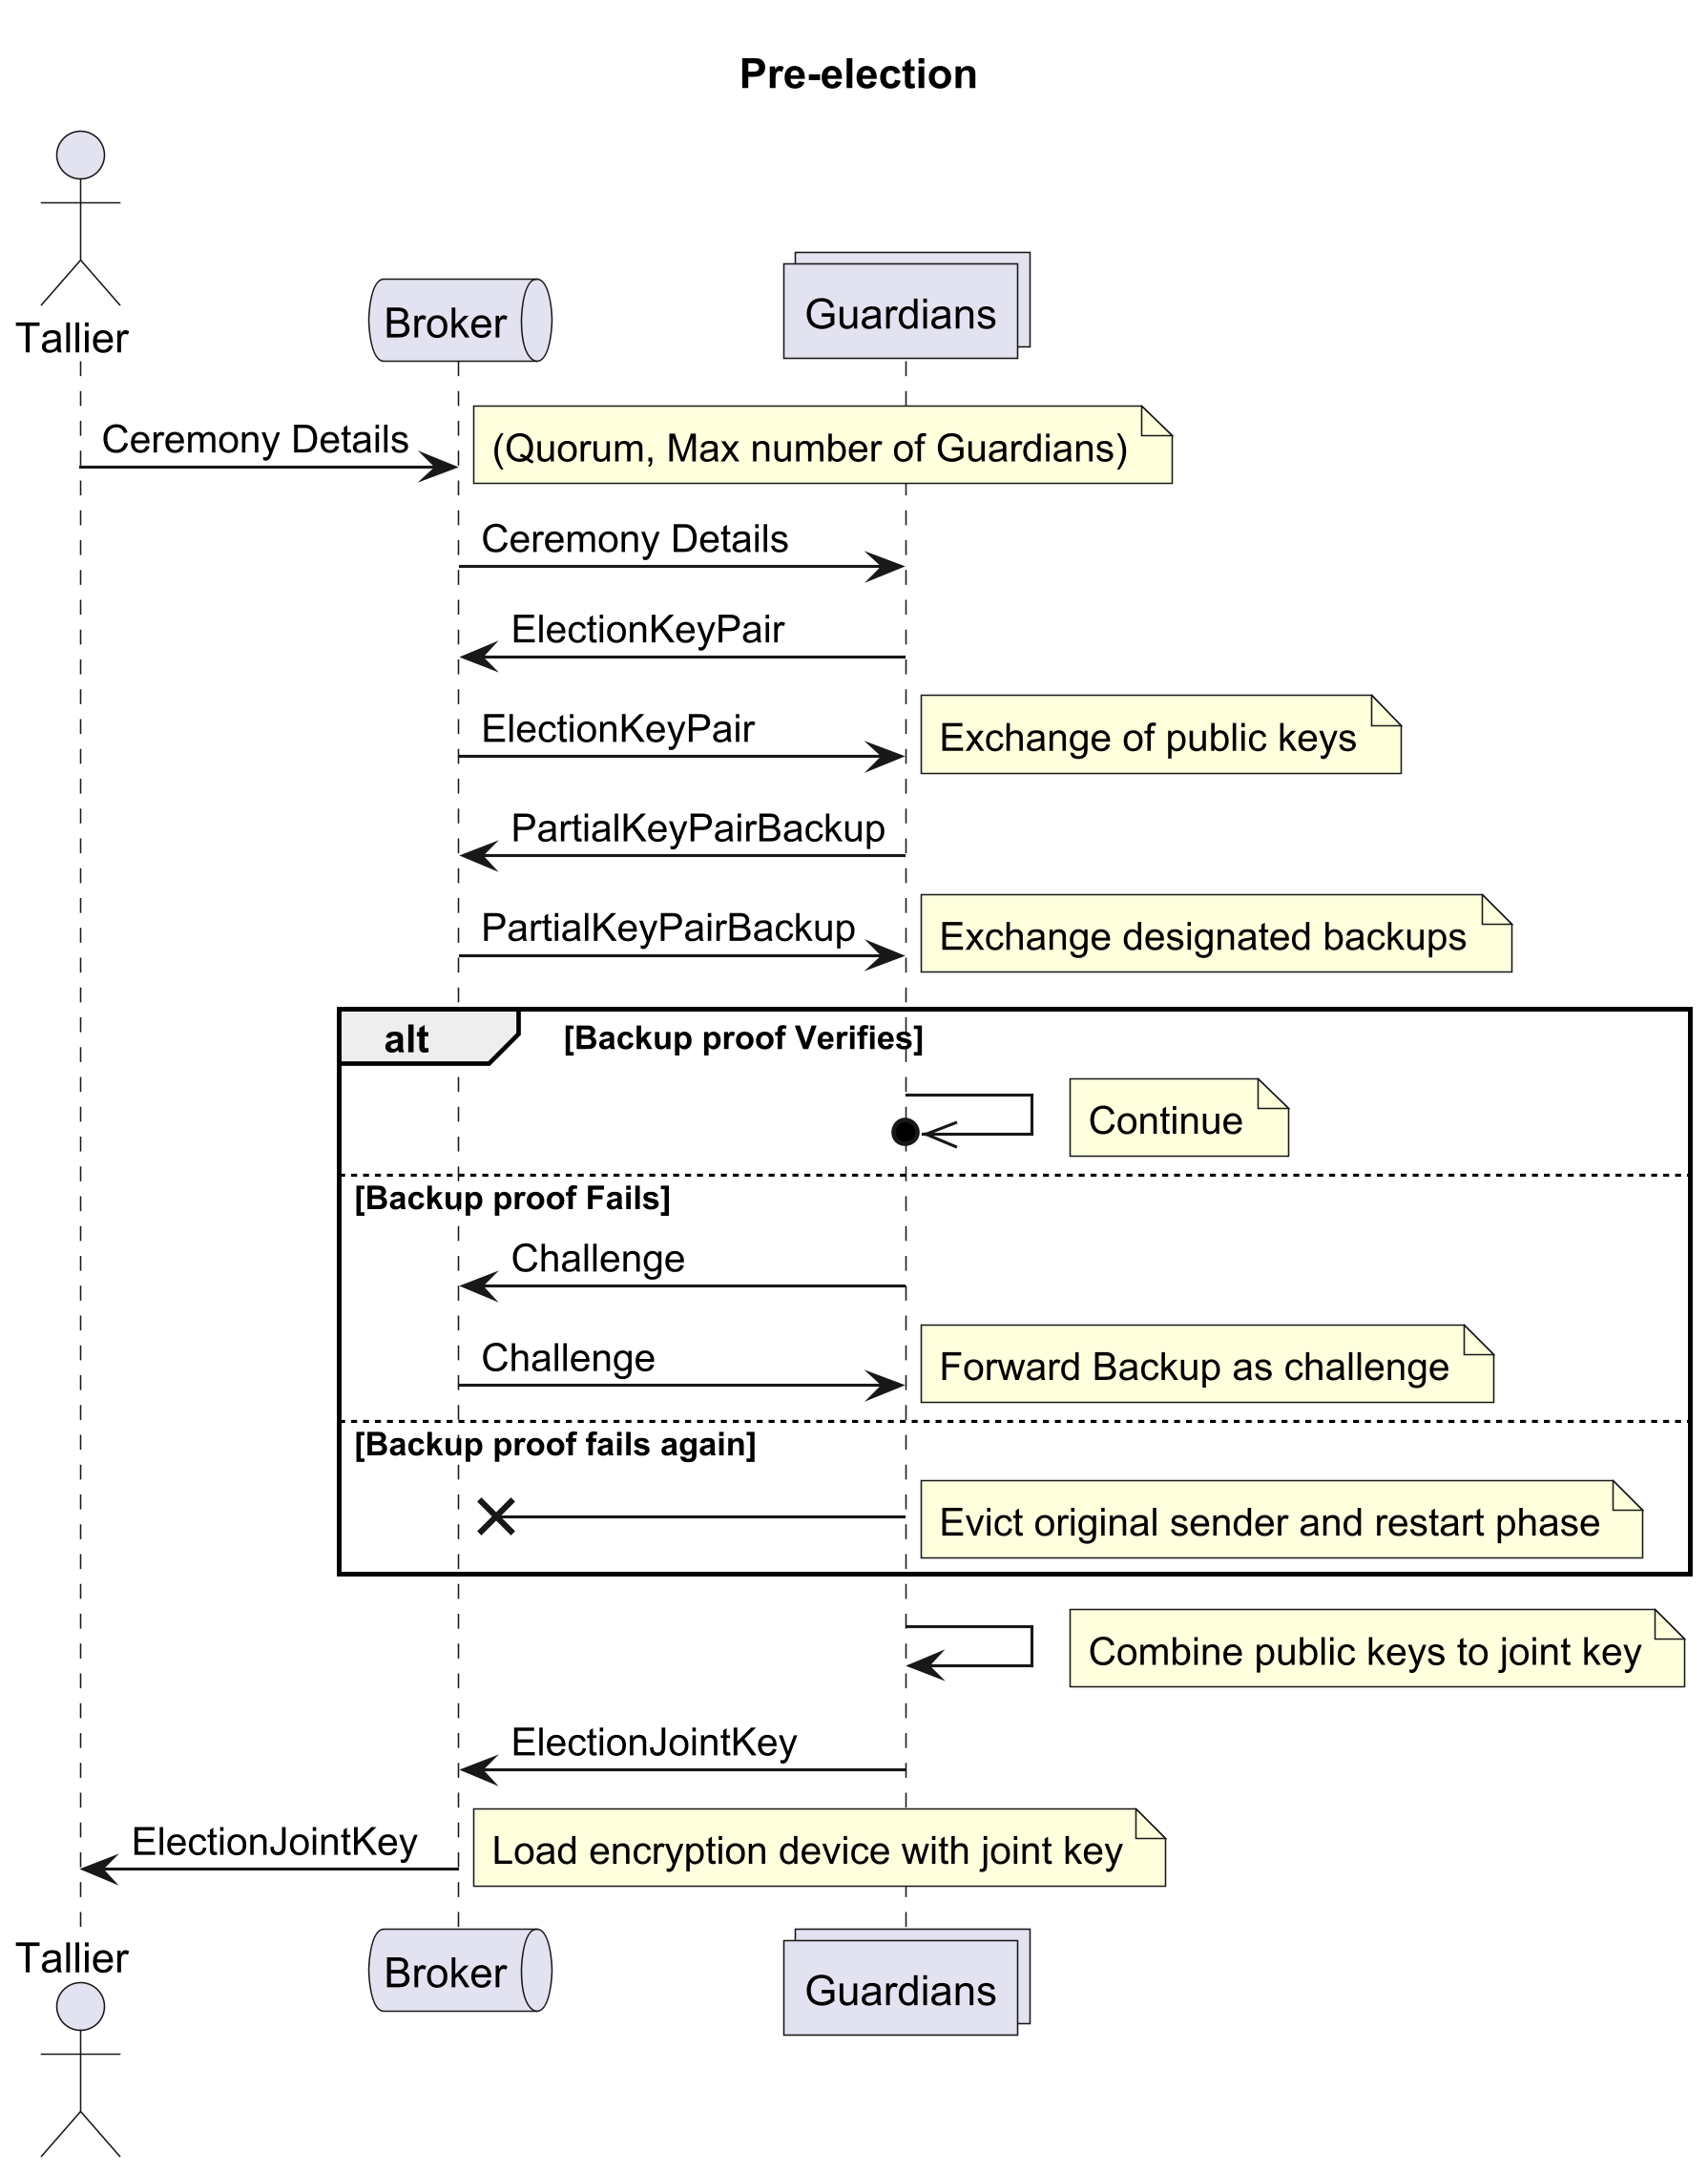
\includegraphics[width=0.7\textwidth]{abbildungen/Diagramme/communication-seq0-mqtt.png}
    \caption{Communication Sequence in the Pre-Election Phase using \ac{MQTT}}\label{fig:mqtt-pre}
\end{figure}

\begin{figure}[ht!]
    \centering
    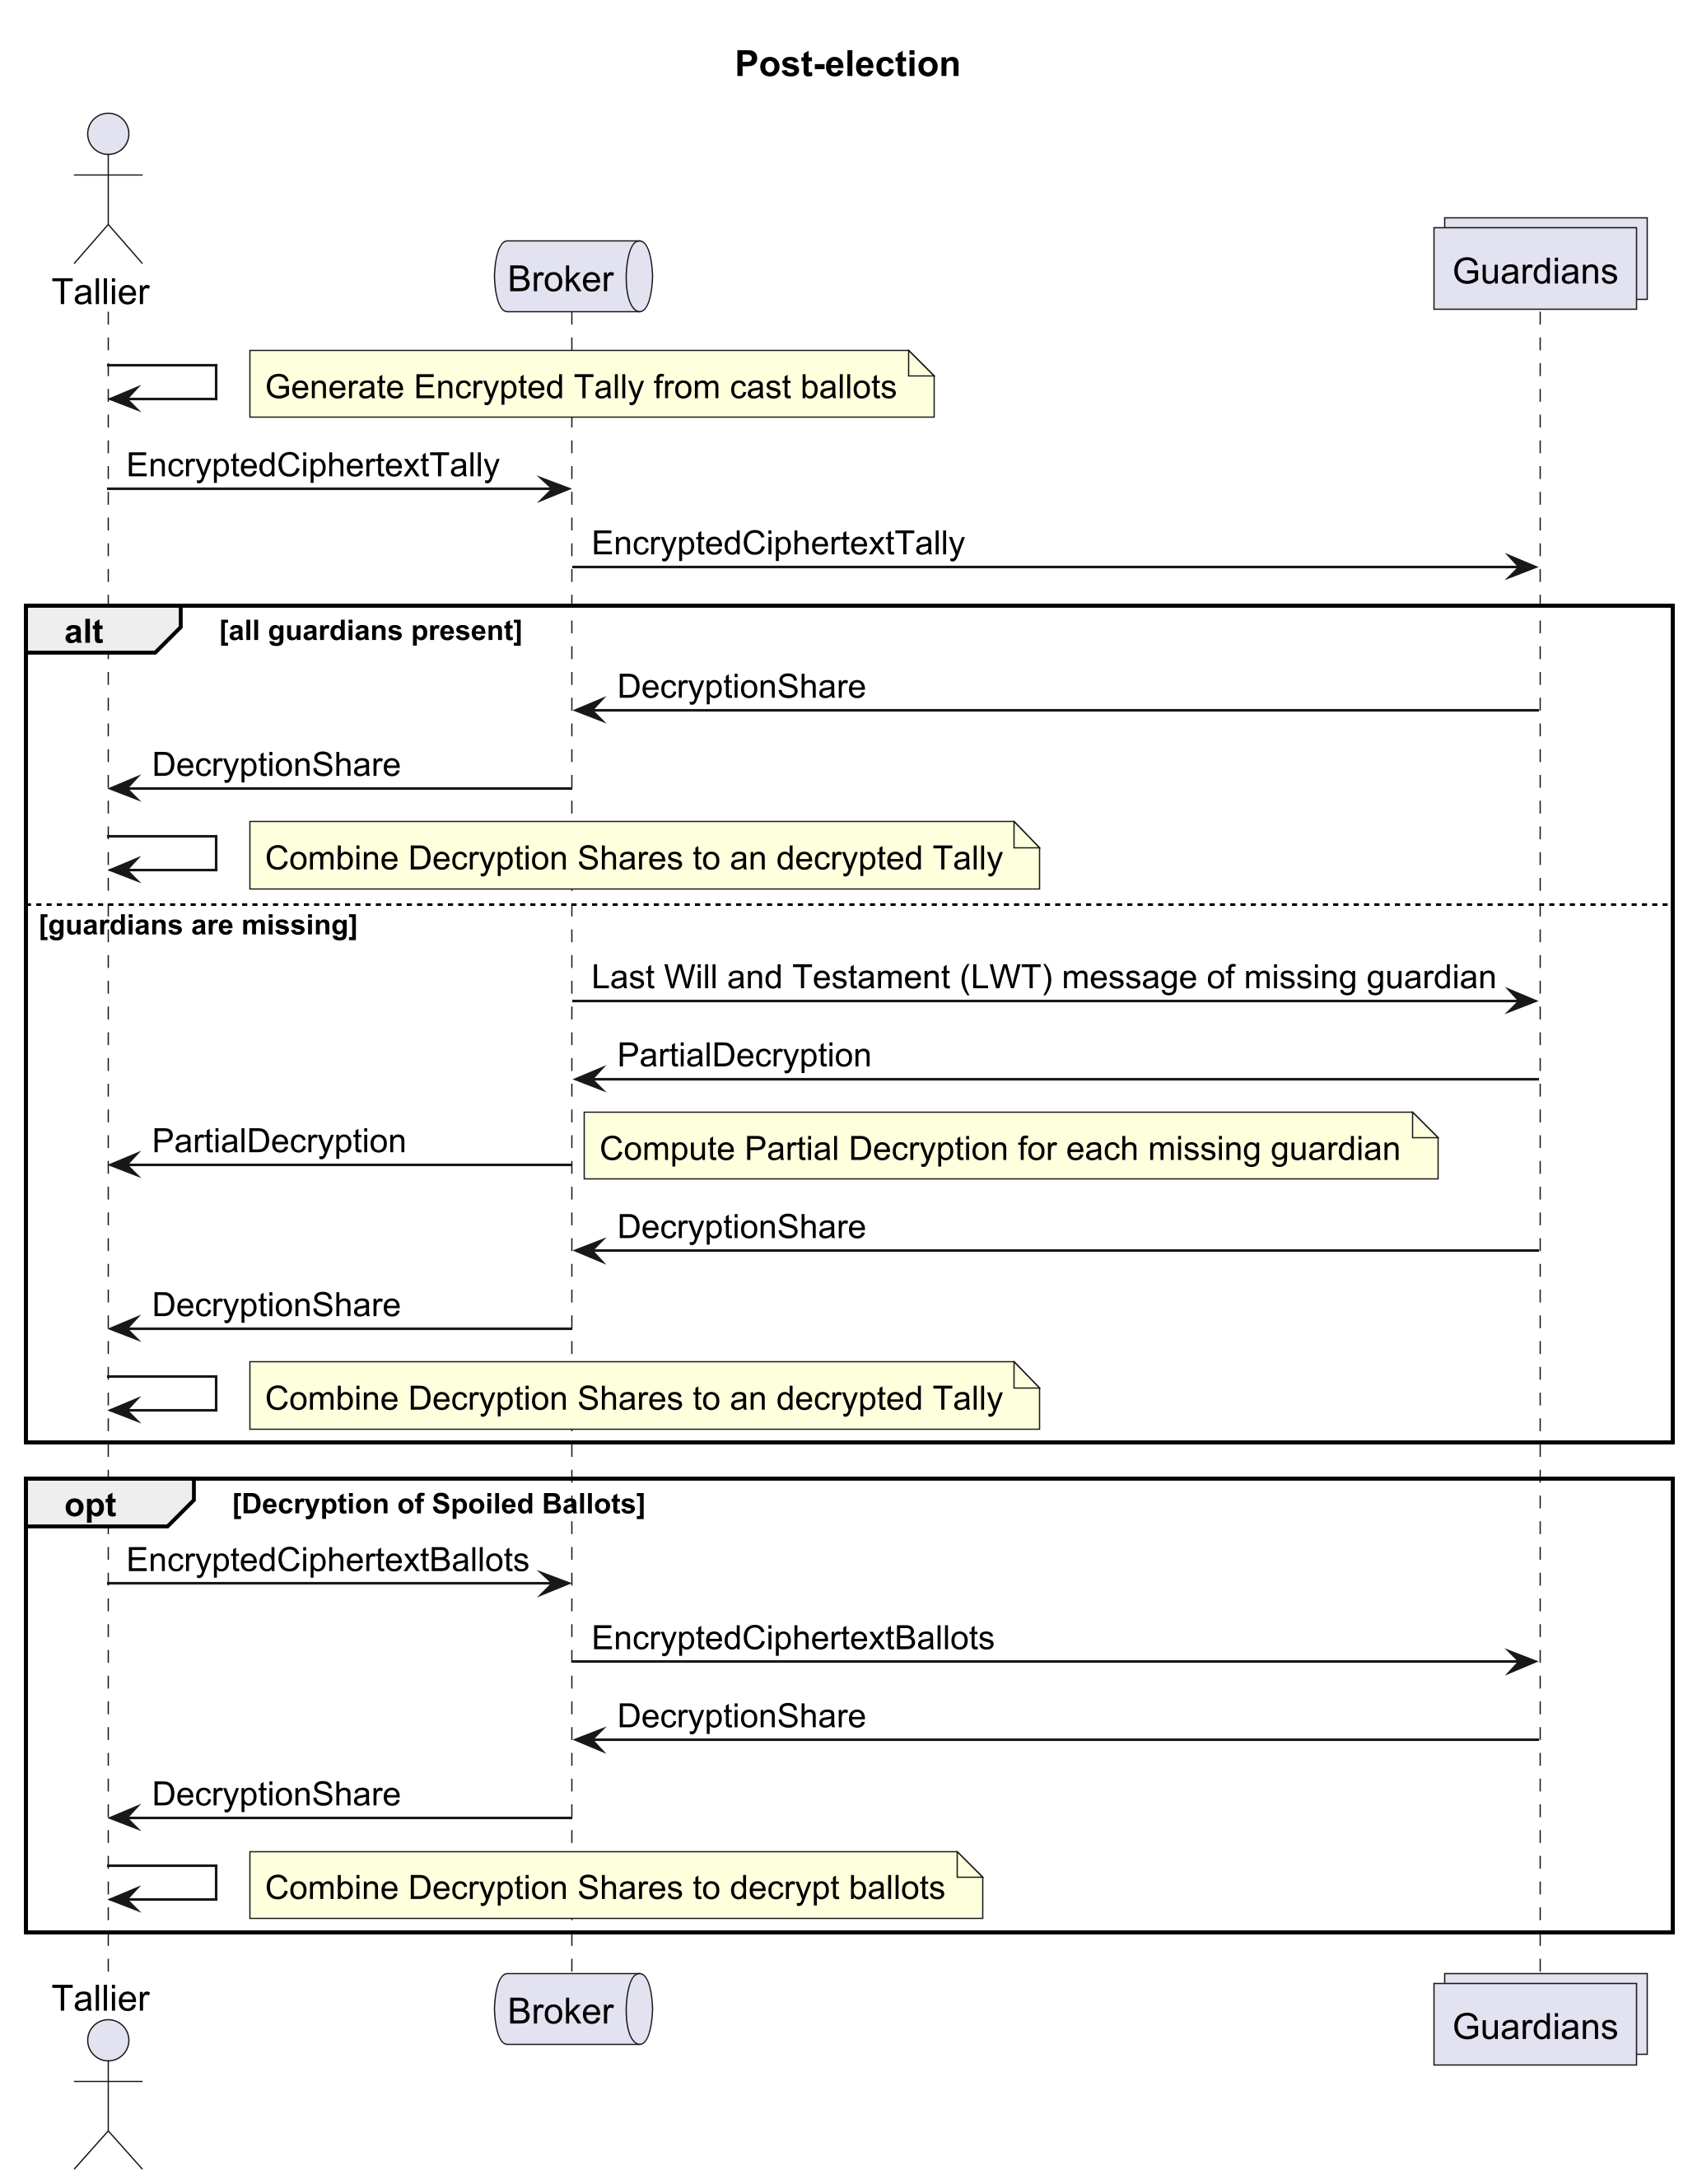
\includegraphics[width=0.7\textwidth]{abbildungen/Diagramme/communication-seq2-mqtt.png}
    \caption{Communication Sequence in the Pre-Election Phase using \ac{MQTT}}\label{fig:mqtt-post}
\end{figure}

Figure \ref{fig:mqtt-pre} shows a sequence diagram of the \ac{MQTT} brokering model, illustrating all entities involved in the key-generation ceremony, including the Tallier, Guardians, and the \ac{MQTT} broker. The \ac{MQTT} broker is running on the Tallier. Both Tallier and Guardians act as publishers and subscribers. During key-generation ceremony, the Guardians programmatically ignore their own public key. For backups, the Guardians ignore all backups that are not meant for them. The \ac{MQTT} specification contains a \textbf{"No Local"} \cite[73]{mqtt-v5.0} subscription option that allows a client to avoid receiving messages it itself has published. However, the ESP32 \ac{MQTT} library does not implement this option \cite[53]{esp-prog}. It is also possible to create one-to-one communication. Guardians could send messages to specific topics that only a specific client is subscribed too. The broker would need to implement some form of access control. In our implementation clients publish to the topics "public\_key", "backups", "ciphertally", "decryption\_share", "ceremony\_details" without any access control. At the end of the key-generation ceremony, the Guardians generate a joint key; the Tallier will simply ignore all other keys sent to it after receiving the first key.

Figure \ref{fig:mqtt-post} shows a sequence diagram of the \ac{MQTT} brokering model, illustrating all entities involved in the decryption phase, including the Tallier, Guardians, and the \ac{MQTT} broker. The case where a Guardian is missing is not implemented in this scenario. This could be addressed through Last Will and Testament message, which allow clients to notify other clients on unexpected disconnects \cite[53]{esp-prog}. The Guardian could then act accordingly. Decrypting spoiled ballots is optional and is not implemented in the current system. The decryption of spoiled ballots is similar to the decryption of the encrypted tally.

To facilitate the sending and receiving of large packets, we set the input and output buffer size of the ESP32 MQTT implementation to 4253 bytes. If this is not set, large packets are sent sequentially by the client, leading to additional overhead.

\section{Network Traffic Analysis}
Network traffic between Tallier and Guardians was captured using Wireshark (4.4.3) by listening to the \ac{AP} interface of the laptop. The \ac{MTU} size of the \ac{AP} is 1500 Bytes. Both Guardians where positioned in close proximity to the laptop. The further clients are from the broker, the longer the travel time of the \ac{MQTT} messages and the higher the latency \cite[20]{protocols}. The traffic was narrowed down by applying a display filter to exclude all non-\ac{MQTT} traffic. The capture focused on the unencrypted communication described in \ref{sec:mqtt-impl}. The workflow is automated, requiring no human interaction. Three captures were taken: one with the number of cast ballots set to 10, another with it set to 100, and the third with it set to 1000 votes. The captures will be refered to as Capture 10, Capture 100, and Capture 1000 respectively. In all capture scenarions, no packet loss occured. Large payloads (e.g., keys/backups) exceeding the \ac{MTU} size are split into multiple TCP segments and reassembled at the receiving end.
\begin{figure}[ht!]
    \centering
    \begin{subfigure}[b]{0.6\textwidth}
        \centering
        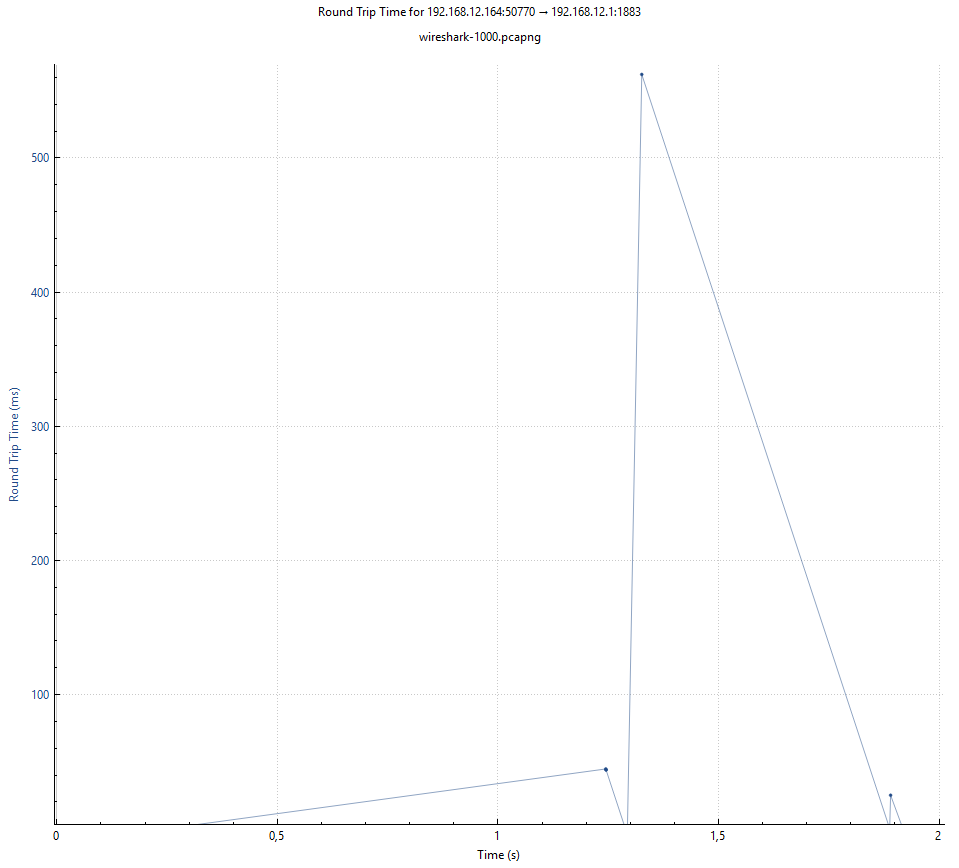
\includegraphics[width=\textwidth]{abbildungen/wireshark/1000-g1.png}
        \caption{\ac{RTT} of Guardian 1 (192.168.12.164) at the start of Capture 1000}
        \label{fig:rtt-g1}
    \end{subfigure}
    \hfill
    \begin{subfigure}[b]{0.6\textwidth}
        \centering
        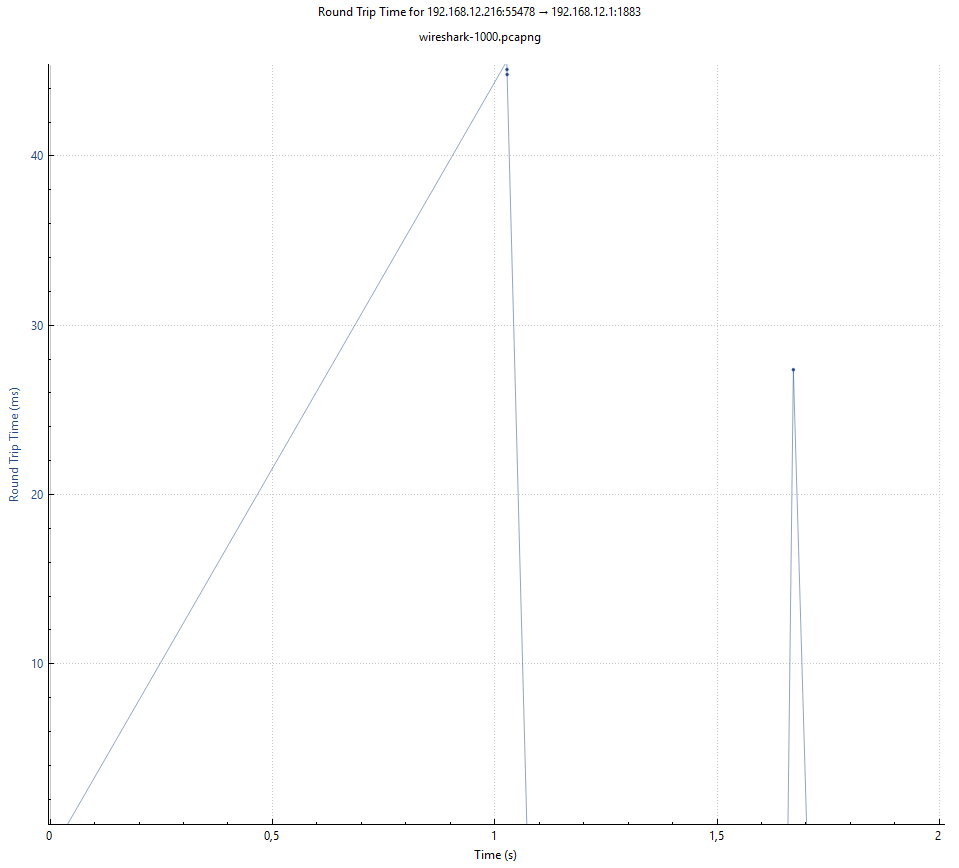
\includegraphics[width=\textwidth]{abbildungen/wireshark/1000-g2.png}
        \caption{\ac{RTT} of Guardian 2 (192.168.12.216) at the start of Capture 1000}
        \label{fig:rtt-g2}
    \end{subfigure}
    \caption{Comparison of \ac{RTT} of Guardians at the start of Capture 1000}
    \label{fig:rtt}
\end{figure}
\begin{figure}[ht!]
    \centering
    \begin{subfigure}[b]{\textwidth}
        \centering
        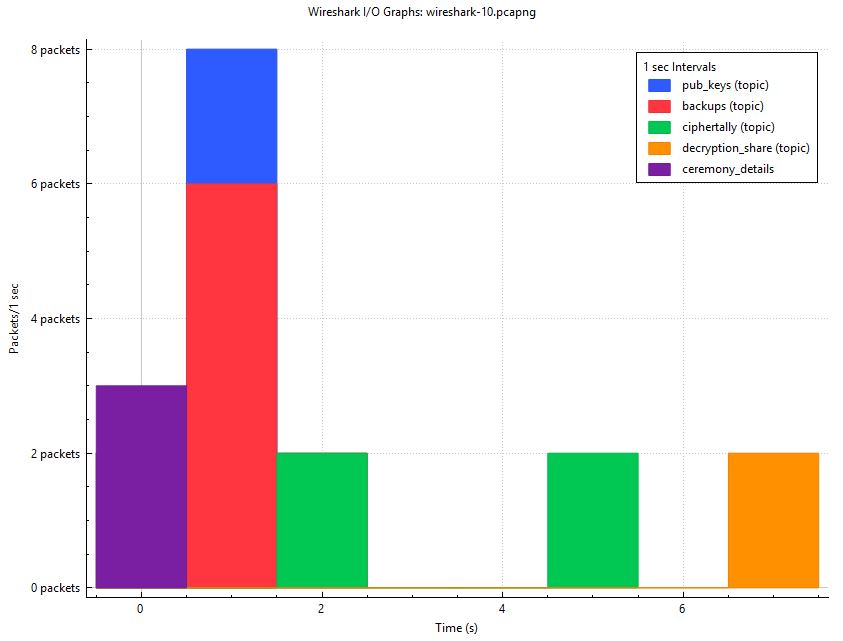
\includegraphics[width=\textwidth]{abbildungen/wireshark/wireshark-10-burst.png}
        \caption{Package rate on specific topics in Capture 10}
        \label{fig:rate-10}
    \end{subfigure}
    \hfill
    \begin{subfigure}[b]{\textwidth}
        \centering
        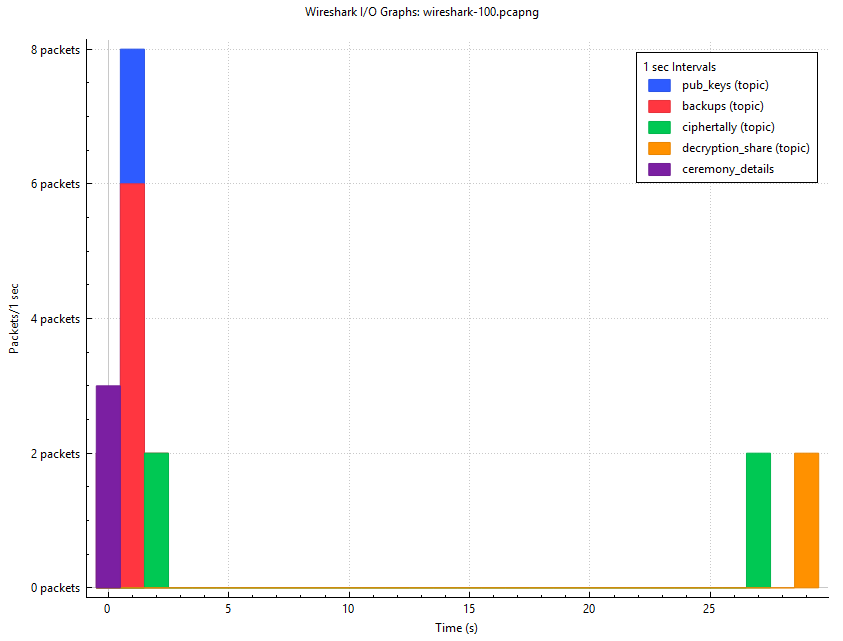
\includegraphics[width=\textwidth]{abbildungen/wireshark/wireshark-100-burst.png}
        \caption{Package rate on specific topics in Capture 100}
        \label{fig:rate-100}
    \end{subfigure}
    \caption{Communication Sequences using MQTT in Different Phases}
    \label{fig:rate}
\end{figure}
\ac{RTT} is the time it takes for a packet to travel from the sender to the receiver and back. \ac{RTT} is a key-metric for measuring network performance. The \ac{RTT} of both Guardians is consisten at around 45ms throughout all captures. However, the \ac{RTT} peaks consistently to over 500ms for Guardian 1 (192.168.12.164) near the beginning of each capture, as seen in Figure \ref{fig:rtt}. This could be due to network congestion at the start of the capture. To identify potential bottlenecks, we analyse the most active topics, as shown in Figure \ref{fig:rate}. The figure excludes packets related to \ac{QoS}. The peak at the beginning of both captures 10 and 100 coincides with peak in \ac{RTT}. The most active topics are the "backups" and "public\_keys" topic. We send a significant number of packets here because clients that send a payload to these topics will receive their own packets again. The throughput could drop significantly as the number of subscriptions increases. As more clients subscribe to topic the number of messages increases \cite[19,21,22]{protocols}. The payload of these packets is also large, measuring 2940 bytes for "public\_keys" and 474 bytes for "backups". Furthermore, payloads send to the topics "public\_keys" and "backups" are transmitted with \ac{QoS} 2. The more clients subscribed to receive a message with \ac{QoS} 2, the greater the overhead on the message broker \cite[11]{protocols}. The payloads sent to the topics "decryption\_share" and "ciphertally" towards the end of the capture are also quite large, but are published with \ac{QoS} 1. The payload size send to the "ciphertally" topic is 2498 bytes, while the payload to the "decryption\_share" topic is 4253 bytes. The \ac{RTT} remained under 45ms for both clients towards the end of the capture.
\begin{figure}[ht!]
    \centering
    \begin{subfigure}[b]{0.45\textwidth}
        \centering
        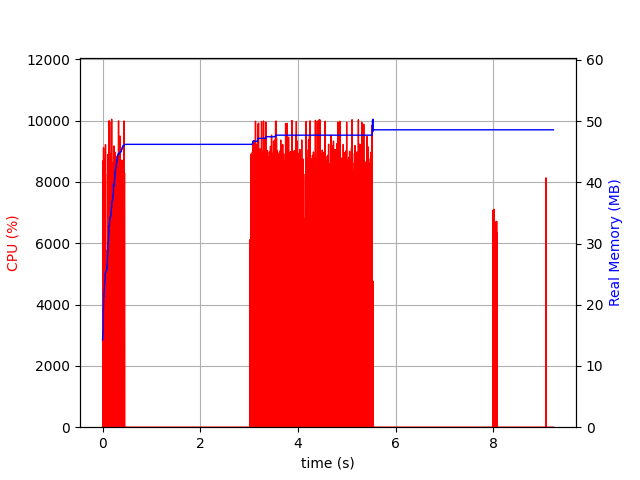
\includegraphics[width=\textwidth]{abbildungen/10.png}
        \caption{Capture 10}
        \label{fig:cpu-10}
    \end{subfigure}
    \begin{subfigure}[b]{0.45\textwidth}
        \centering
        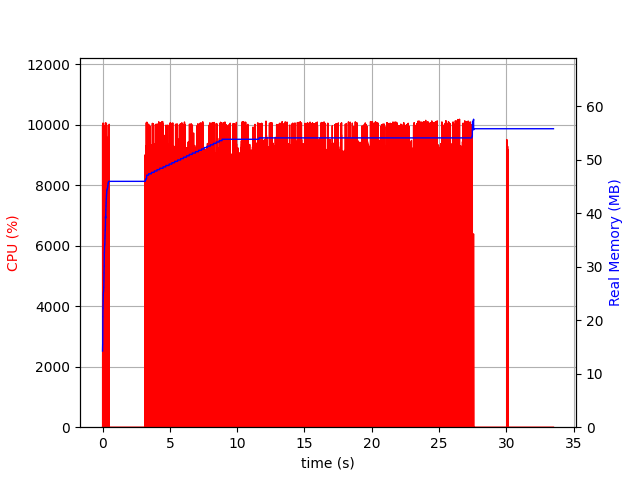
\includegraphics[width=\textwidth]{abbildungen/100.png}
        \caption{Capture 100}
        \label{fig:cpu-100}
    \end{subfigure}
    \begin{subfigure}[b]{\textwidth}
        \centering
        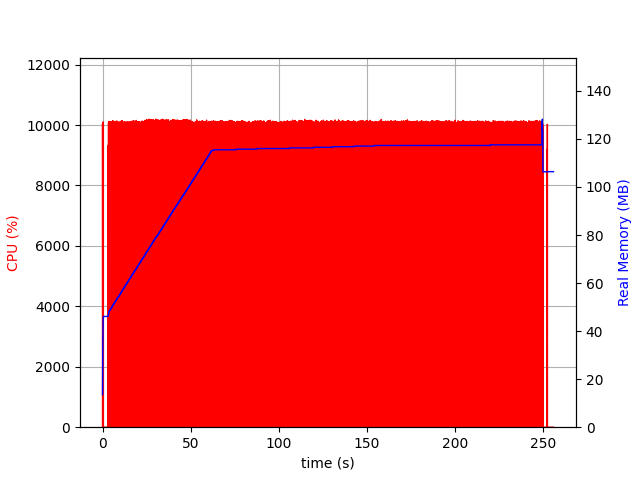
\includegraphics[width=\textwidth]{abbildungen/1000.png}
        \caption{Capture 1000}
        \label{fig:cpu-1000}
    \end{subfigure}
    \caption{Tallier CPU and Memory utilisation in Capture 10, 100, and 1000, plotted with the python package psrecord}
    \label{fig:cpu}
\end{figure}
\begin{table}[ht!]
    \centering
    \begin{tabular}{|c|c|c|c|}
        \hline
        \textbf{Capture} & \textbf{Duration (s)} & \textbf{G1->Tallier (Bits/s)} & \textbf{G2->Tallier (Bits/s)} \\
        \hline
        10 & 7.54 & 10086 & 10146 \\
        \hline
        100 & 29.57 & 2572 & 2587 \\
        \hline
        1000 & 251.90 & 305 & 305 \\
        \hline
    \end{tabular}
    \caption{Throughput and Duration of Captures, G1 and G2 are the Guardians}
    \label{tab:throughput_duration}
\end{table}
Wiresharks conversation statistic shows us the throughput of the capture, as detailed in Table \ref{tab:throughput_duration}. The data volume per capture is consistent at approximately 20 KB, but the transmission frequency varies. Capture 10 exhibits a high-frequency burst with a duration of 7.54s. Capture 100 has a duration of 29.57 seconds, while Capture 1000 is a slow transmission with a duration of 251.90 seconds. Each capture transmits roughly the same data volume but spreads it out over longer periods.  Comparing this to the packet rate on specific topics between different captures, it becomes evident that the most time spent is after key-generation and before decryption, during which the Guardians are idling. The increase in duration correlates with the increase in votes. This is due to the processing time required by the Tallier, which needs to homomorphically encrypt the votes before sending the ciphertally. The Tallier's CPU and memory utilisation is plotted in Figure \ref{fig:cpu}. Memory usage peaks at 50 MB for Capture 10. Slightly increases in Capture 100, and increases to over 120 MB in Capture 1000. The computation time increases significantly with the number of votes, indicating that the homomorphic encryption performed by the Tallier is the major bottleneck of the system.

%Befehl um sämtliche Literatur im Literaturverzeichnis aufzuführen
\nocite{*}

